%% The following is a directive for TeXShop to indicate the main file
%%!TEX root = diss.tex

\chapter{A Taxonomy of 3D Reconstruction}
\label{ch:3DRecon_Taxo}
Existing taxonomies of 3D reconstruction techniques generally focus on one category of techniques: the Multi-view Stereo taxonomy in~\cite{seitz2006comparison} proposed classification of MVS algorithms from various perspectives. Reviews of Structured Light techniques generally classify techniques based on the type of projection pattern used~\cite{geng2011structured, salvi2004pattern}. Photometric Stereo algorithms are classified by the assumptions or generalizations made, for instance, unknown/known reflectance, unknown/known light conditions (uncalibrated/calibrated), etc~\cite{shi2016benchmark}. These frameworks provide a way to categorize intra-category algorithms, but is unsuitable to evaluate the performance of inter-category algorithms. Furthermore, the algorithms under consideration are targeted at a limited categories of objects. It's well known that these algorithms are highly likely to fail on other categories of objects, and this knowledge of algorithmic applicability is largely empirical, with each algorithm roughly maps to a problem domain that is poorly defined. Thus we need a more object-centered approach to the taxonomy so that a more precise mapping is available.

It's crutial to understand where algorithms perform well and where they fail when designing an application for reconstruction. Under the previous framework of taxonomy, this knowledge is largely empirical, with each algorithm mapped roughly to a sub-volume in the problem space. However, this mapping is ambigueous, \ie the sub-space is not well defined, and also too general, \ie algorithm within the same category cannot be effectively distinguished. To overcome this limitation, we need to 1). propose a well-defined problem space; 2). bypass the algorithmic details and focus on properties that are not intuitive to understand and perceive.

The taxonomy proposed in this chapter defines the 3D reconstruction techniques from a object-centered viewpoint, \ie categorize algorithm based on object class. This taxonomy transforms the 3D reconstruction problem from one requiring knowledge and expertise of specific algorithms in terms of how and when to use them, to one requiring knowledge of the visual and geometric properties of the target object. We first propose a $n-$dimensional problem space where each dimension is 

\section{New Perspective}
Most previous taxonomies categorize algorithms based on the algorithmic details. However, this approach 1). gives very little insight as what conditions does a specific algorithm work well; 2). requires vision knowledge to understand and use these algorithms.

The new perspective approaches the taxonomy from a different angle.

\section{Problem Space}
The dimension of the problem space should be orthogonal, and 

\section{Object class}
In Figure~\ref{fig:obj_class} (a), we show a taxonomy of object classes with different material and shape properties. There are in total $3\times 3\times 2\times4\times 2\times 5 = 720$ classes of objects, which still don't fully capture the variations exhibited by real world objects, for instance, effects such as occlusion, discontinuity, emission, etc are not considered. Most techniques that have been developed over the past decades can only tackle a subset of all possible object classes, with a focus on opaque, diffuse objects. For specular, refractive, and translucent or transparent objects, only very specialized algorithms are applicable for reconstruction~\cite{ihrke2010transparent}.

To make the problem tackleable, only six classes of objects are being investigated in depth. The reasoning behind the selected object classes is solely based on the [popularity] of the class. See Figure~\ref{fig:obj_class} (b) for the six classes of objects.
\begin{figure}[!htbp]
\centering
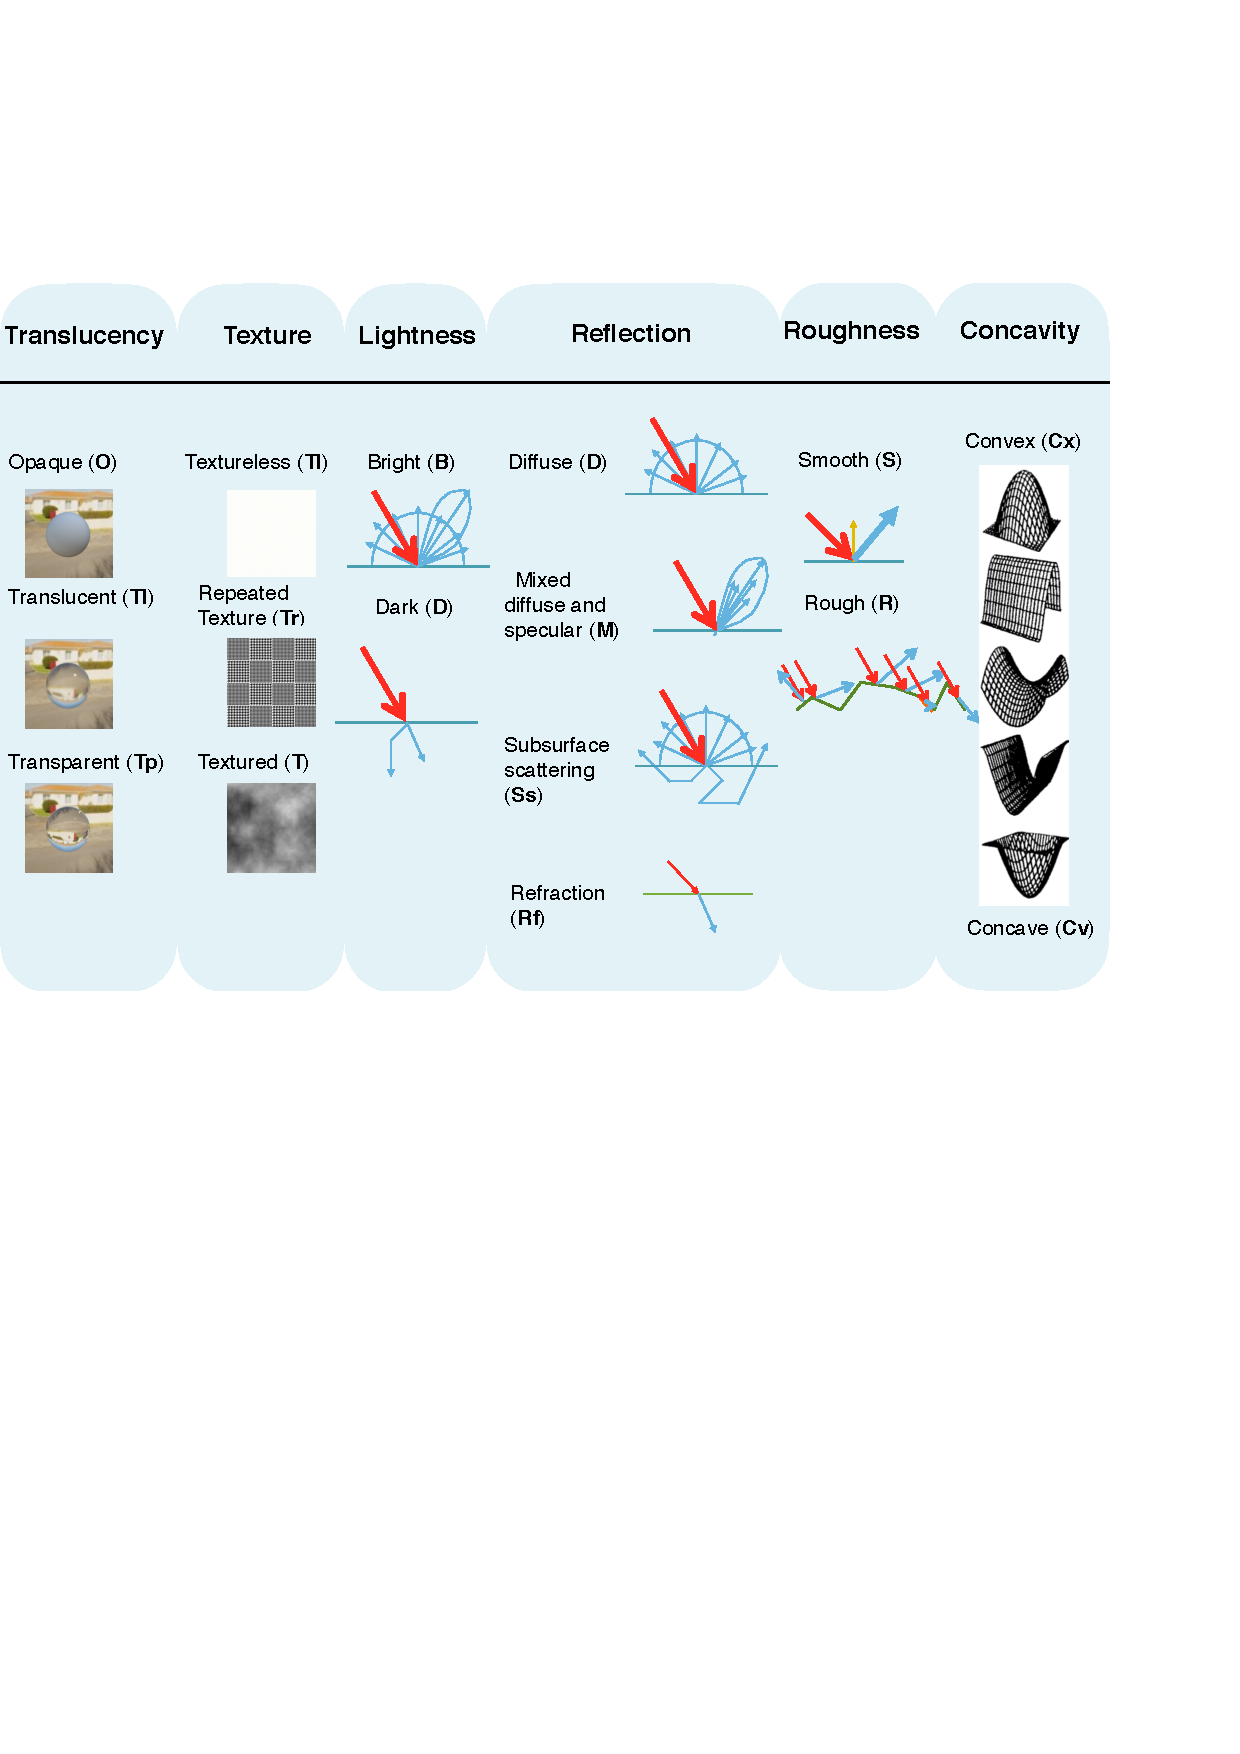
\includegraphics[width=0.8\textwidth]{taxo/obj_class}\\
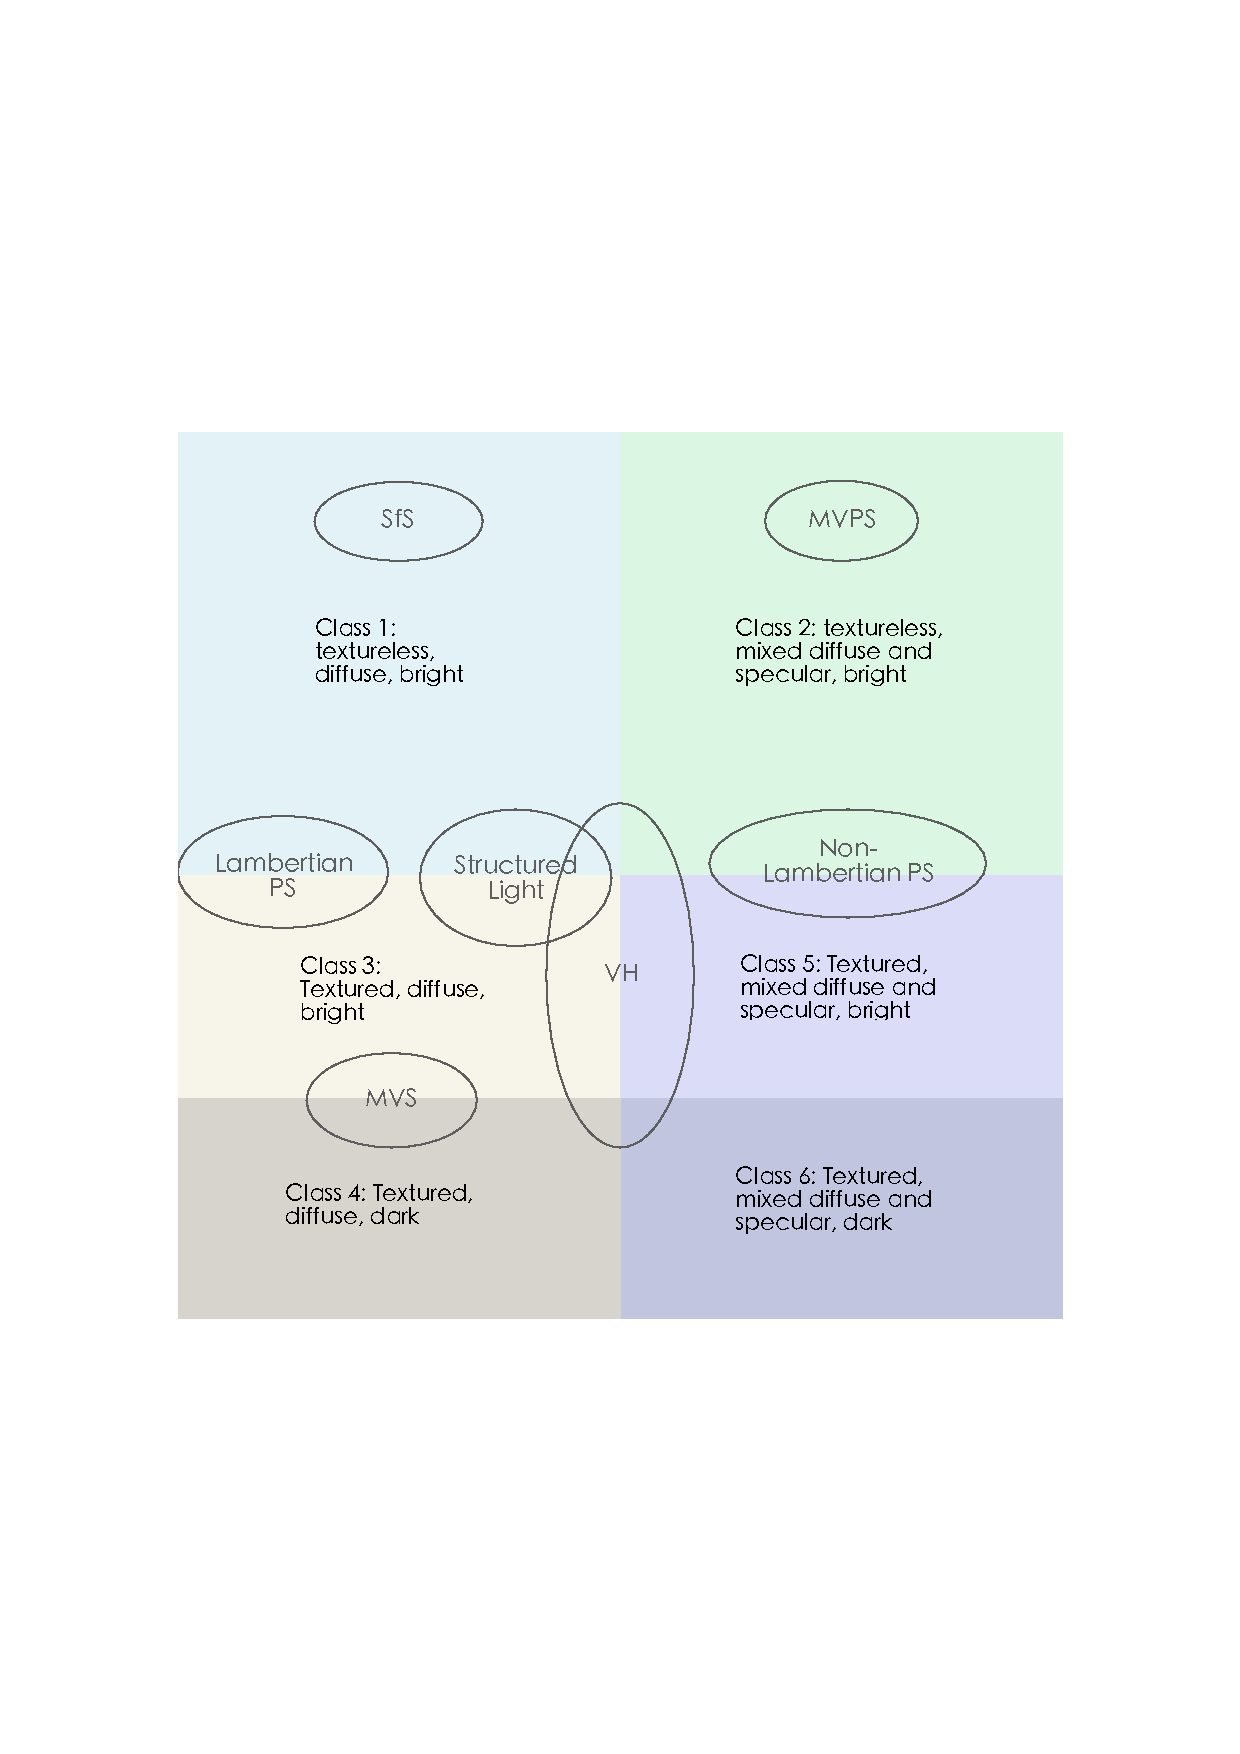
\includegraphics[width=0.8\textwidth]{taxo/six_class}\\
\caption{\textit{Top}: A list of properties for object classes. \textit{Bottom}: Six object classes of interest. Only texture, lightness, and reflectance are consider. Properties not consider are set as follows: opaque, rough (for Lambertian)/smooth (for Non-Lambertian), low concavity.}
\label{fig:obj_class}
\end{figure}

Here is a list of algorithms we will look into in depth, a summary is list in Table\ref{tab:class_algo}.
\begin{table}[!htbp]
  \centering
  \begin{tabular}{l||l}
  \hline
  \textbf{Algo. class} & \textbf{Technique}\\
  \hline
  SfS & Horn~\cite{horn1970shape}\\
  MVS & Furukawa~\cite{furukawa2010accurate}, Goesele~\cite{goesele2006multi}, Vogiatzis~\cite{vogiatzis2007multiview}, \\
      & Hern{\'a}ndez~\cite{esteban2004silhouette}, Faugeras~\cite{faugeras2002variational}\\
  Lamberian PS & Woodham~\cite{woodham1980photometric}, Hayakawa~\cite{hayakawa1994photometric}, Belhumeur~\cite{belhumeur1999bas}, \\
      & Alldrin~\cite{alldrin2007resolving}\\
  Non Lambertian PS & Coleman~\cite{coleman1982obtaining}, Barsky~\cite{barsky20034}, Schluns~\cite{schluns1993photometric}, Sato~\cite{sato1994temporal}, \\
      & Mallick~\cite{mallick2005beyond}, Alldrain~\cite{alldrin2008photometric}, Goldman~\cite{goldman2010shape}, Silver~\cite{silver1980determining}, \\
      & Hertzmann~\cite{hertzmann2005example}, Zickler~\cite{zickler2002helmholtz}\\
  % MVPS & \checkmark & \\
  SL & Inokuchi~\cite{inokuchi1984range}\\
  VH & Szeliski~\cite{szeliski1993rapid}, Matusik~\cite{matusik2002efficient}, Tarini~\cite{tarini2002marching}\\
  \hline
  \end{tabular}
  \caption{Selected algorithms from each class of algorithms}
  \label{tab:class_algo}
\end{table}

\section{Class 1}
\label{sec:class_1}
In this section, we discuss techniques for reconstructing bright, textureless, and diffuse surfaces. The reconstruction of this type of surfaces is complicated by the fact that there is no spatial information available for stereo correpondence searching due to the lack of texture, thus making passive stereo based methods unavailable. Textureless and diffuse surface also indicates uniform reflectance, \ie uniform diffuse albedo. The conditions under which each categories of algorithms would work or fail are listed in Table~\ref{tab:class_1}.
\begin{table}[!ht]
  \centering
  \begin{tabular}{l*{3}{c}}
  \hline
  \textbf{Technique} & Textureless & Bright & Lambertian\\
  \hline
  SfS & \checkmark & \checkmark & \checkmark\\
  MVS & \ding{55} & \checkmark & \checkmark\\
  Lamberian PS & \checkmark & \checkmark & \checkmark\\
  Non Lambertian PS & \checkmark & \checkmark & \ding{55}\\
  MVPS & \checkmark & \checkmark & \checkmark\\
  SL & \checkmark & \checkmark & \checkmark\\
  VH & \checkmark & \checkmark & \checkmark\\
  \hline
  \end{tabular}
  \caption{Categories of algorithm that are applicable for object class 1.}
  \label{tab:class_1}
\end{table}

\subsection{SfS}
Shape from Shading, first proposed by~\citeauthor{horn1970shape} is targeted specifically for known isotropic Lambertian surfaces. By assuming orthographic projection, and known light source intensity and direction, surface orientation can be estimated from the shading variations.

% To obtain a reflectance map, the system is calibrated using a sphere having a constant surface reflectance factor. Shape can be determined for only those objects having reflectacne properties identical to the calibration sphere.

\subsection{Lambertian PS: uniform reflectance}
The traditional Photometric Stereo can be considered as an extenstion of the original Shape from Shading, which incorporates additional light sources to eliminate ambiguity~\cite{woodham1980photometric}. The surface orientation can be retrieved from using only two images.

To avoid the tedious process of light calibration, Silver~\cite{silver1980determining} proposed a look-up scheme that relies on reflectance object with the same reflectance as the target, a uniform Lambertian surface in this case. This approach can be applied to surface with non-Lambertian reflectance, and varying colour or material, see Section~\ref{sec:class_2} for non-Lambertian surfaces, and Section~\ref{sec:class_4},~\ref{sec:class_5} for surfaces with varying colour/material.

\subsection{SL}
For stereo correspondence based methods, actively projected patterns have to be used for the lack of surface texture. Since the surface is diffuse, there is no specular reflection to cause severe noise.
% The constraints and formulations of algorithms for object class 1 are summarised in Table~\ref{tab:summary_class_1}.
% \begin{table}[h]
%   \centering
%   \begin{tabular}{l*{3}{c}}
%   \hline
%   \textbf{Technique} & Calibrated & Reflectance & Algorithm\\
%   \hline
%   Horn~\cite{horn1970shape} & Yes & Lambertian & Characteristic strips\\
%   Woodham~\cite{woodham1980photometric} & Yes & Lambertian & $N = IL^{+}$\\
%   Hayakawa~\cite{hayakawa1994photometric} & No & Lambertian & \\
%   Belhumeur~\cite{belhumeur1999bas} & No & Lambertian & \\
%   Alldrin~\cite{alldrin2007resolving} & No & Lambertian & resolve the GBR ambiguity based on minimization of the entropy of the recovered albedos\\
%   Inokuchi~\cite{inokuchi1984range} & Yes & Lambertian & Triangulation\\
%   \hline
%   \end{tabular}
%   \caption{Summary of constraints and formulations of algorithms for object class 1.}
%   \label{tab:summary_class_1}
% \end{table}

\section{Class 2}
\label{sec:class_2}
This section discusses the reconstruction of bright, textureless, non-Lambertian surfaces. The specular surfaces reflect light in a single direction which follows the law of reflection, thus the appearance changes as the viewpoint changes, which makes the correspondence search in these regions unreliable. Thus textureless and non-Lambertian properties rule out stereo based techniques.  Textureless also indicates that the surface is composed of the same material thus the albedo is uniform across the surface. The conditions under which each categories of algorithms would work or fail are listed in Table~\ref{tab:class_2}.
\begin{table}[h]
  \centering
  \begin{tabular}{l*{3}{c}}
  \hline
  \textbf{Technique} & Textureless & Bright & Non-Lambertian\\
  \hline
  SfS & \checkmark & \checkmark & \ding{55}\\
  MVS & \ding{55} & \checkmark & \ding{55}\\
  Lambertian PS & \checkmark & \checkmark & \ding{55}\\
  Non-Lambertian PS & \checkmark & \checkmark & \checkmark\\
  MVPS & \checkmark & \checkmark & \checkmark\\
  SL & \checkmark & \checkmark & \ding{55}\\
  VH & \checkmark & \checkmark & \checkmark\\
  \hline
  \end{tabular}
  \caption{Categories of algorithm that are applicable for object class 2.}
  \label{tab:class_2}
\end{table}

\subsection{Non-Lambertian PS: uniform reflectance}
This section considers techniques that deal with surfaces composed of the same material, \ie \textit{uniform albedo}. Techniques that can deal with spatially varying reflectance can generally be adapted to deal with surfaces of uniform reflectance. Thus refer to Section~\ref{sec:class_5} for more techniques that are designed for surfaces of spatially-varying reflectance.

As discussed briefly in Section~\ref{sec:class_1}, we can also use a non-Lambertian \textit{reference objects}. The method is first proposed by~\citeauthor{silver1980determining} and later by~\citeauthor{hertzmann2005example}.
% \begin{table}[h]
%   \centering
%   \begin{tabular}{l*{3}{c}}
%   \hline
%   \textbf{Technique} & Calibrated & Reflectance & Algorithm\\
%   \hline
%   Coleman~\cite{coleman1982obtaining} & Yes & specular lobe & Outlier\\
%   Barsky~\cite{barsky20034} & Yes & specular lobe & Outlier\\
%   Schluns~\cite{schluns1993photometric} & Yes & specular lobe & 
%   Separate D/S\\
%   Sato~\cite{sato1994temporal} & Yes & specular lobe & Separate D/S\\
%   Mallick~\cite{mallick2005beyond} & Yes & specular lobe & Separate D/S\\
%   Alldrain~\cite{alldrin2008photometric} & Yes & bi-variate function & Yes\\
%   Goldman~\cite{goldman2010shape} & Yes & Isotropic Ward model & Yes\\
%   Silver~\cite{silver1980determining} & No & Reference object(s) & Orientation consist\\
%   Hertzmann~\cite{hertzmann2005example} & No & Reference object(s) & Orientation consist\\
%   Zickler~\cite{zickler2002helmholtz} & Yes & Physical properties & Helmholtz reciprocity\\
%   \hline
%   \end{tabular}
%   \caption{Summary of Non-Lambertian Photometric Stereo assumptions and formulations}
%   \label{tab:summary_class_2}
% \end{table}

\section{Class 3}
\label{sec:class_3}
This section deals with bright, textured, Lamberian surfaces. Multi-view stereo can use the Lambertian, textured surface to reconstruct a (quasi-)dense model. The conditions under which each categories of algorithms would work or fail are listed in Table~\ref{tab:class_3}.
\begin{table}[h]
  \centering
  \begin{tabular}{l*{3}{c}}
  \hline
  \textbf{Technique} & Textured & Bright & Lambertian\\
  \hline
  SfS & \ding{55} & \checkmark & \checkmark\\
  MVS & \checkmark & \checkmark & \checkmark\\
  Lamberian PS & \checkmark & \checkmark & \checkmark\\
  Non Lambertian PS & \checkmark & \checkmark & \ding{55}\\
  MVPS & \ding{55} & \checkmark & \checkmark\\
  SL & \ding{55} & \checkmark & \checkmark\\
  VH & \checkmark & \checkmark & \checkmark\\
  \hline
  \end{tabular}
  \caption{Categories of algorithm that are applicable for object class 3.}
  \label{tab:class_3}
\end{table}
% \begin{itemize}
% \item \textbf{Scene representation}: \textit{3D grid}, \textit{point cloud}, \textit{polygon mesh}, and \textit{depth map};
% \item \textbf{Photo-consistency measure}: \textit{scene space}, \textit{image space};
% \item \textbf{Visibility model}: \textit{geometric}, \textit{quasi-geometric}, and \textit{outlier-based approach};
% \item \textbf{Shape prior}: \textit{minimal surface}, \textit{maximal surface}, and \textit{local smoothness};
% \item \textbf{Algorithm}: \textit{extraction from a 3D volume}, \textit{surface/volume evolution}, \textit{seed point propagation}, \textit{per-view depth map reconstruction};
% \item \textbf{Initialization}: \textit{bounding box}, \textit{range of depth/disparity}.
% \end{itemize}
% We summarize the conditions of these algorithms in Table~\ref{tab:class_3}
% \begin{table}[h]
%   \centering
%   \begin{tabular}{l*{1}{c}}
%   \hline
%   \textbf{Technique} & Algorithm \\
%   \hline
%   Furukawa~\cite{furukawa2010accurate} & Seed propagation\\
%   Goesele~\cite{goesele2006multi} & Depth map estimation\\
%   Vogiatzis~\cite{vogiatzis2007multiview} & 3D grid extraction\\
%   Hern{\'a}ndez~\cite{esteban2004silhouette} & \\
%   Faugeras~\cite{faugeras2002variational} & Level-set evolution\\
%   \hline
%   \end{tabular}
%   \caption{Summary of MVS reconstruction approach.}
%   \label{tab:class_3}
% \end{table}

\subsection{MVS}
The diffuse and textured surface is most suitable for MVS algorithms. However, active technique could work, but the surface texture might interfere with the encoding process thus making the reconstruction inaccurate. \citeauthor{furukawa2008high} use wide-baseline stereo matching to recover the 3D coordinates of salient feature points, then shrink a visual hull model so that the recovered points lie on its surface, then refine the result using energy minimization. \citeauthor{goesele2006multi} compute a depth map from each camera viewpoint (similar to [31]) and merge the results using VRIP [62]. \citeauthor{esteban2004silhouette} first com- pute a depth map from each camera viewpoint and merge the results into a cost volume. They then iteratively deform a mesh, initialized at the visual hull, to find a minimum cost surface in this volume, also incorporating terms to fit silhouettes. Kolmogorov and Zabih [35] compute a set of depth maps using multi-baseline stereo with graph cuts, then merge the results into a voxel volume by computing the intersections of the occluded volumes from each viewpoint. \citeauthor{faugeras2002variational} compute a minimum cost surface by evolving a surface in a level-set frame-work, using a prediction-error measure. \citeauthor{vogiatzis2007multiview} compute a correlation cost volume in the neighborhood of the visual hull. A minimum-cost surface is then computed using volumetric min-cut.

\subsection{Lambertian PS: non-uniform reflectance}
Visual texture can be thought of as a pattern or variance of intensity appearing on an object's surface. In this thesis, the visual texture will be considered as resulting from non-uniform surface albedo. This section discusses techniques that deal with surfaces of \textit{spatially varying albedo}.

The original photometric stereo can also be used for surfaces with spatially-varying albedo. The albedo-scaled normal can be first estimated as usual, then the albedo is retrieved as the magnitude of the scaled normal~\cite{woodham1980photometric}. This method requires three instead of two images.

To avoid the tedious process of light calibration, \textit{uncalibrated photometric stereo} has been proposed. One approach used six or more pixels with the same albedo, and was able to solve for normals up to a rotation ambiguity\cite{hayakawa1994photometric}. It can be further proved that a 3-parameter subset of these transformations, known as the Generalized Bas-Relief (GBR) ambiguity, preserve surface integrability~\cite{belhumeur1999bas}. Thus, given three or more imges of a Lambertian object acquired under light sources of unknown direction and strength, the surface can be reconstructed up to GBR transformation by enforcing surface integrability, see Figure~\ref{fig:gbr} for the effect of GBR-ambiguity.
\begin{figure}[!htbp]
\centering
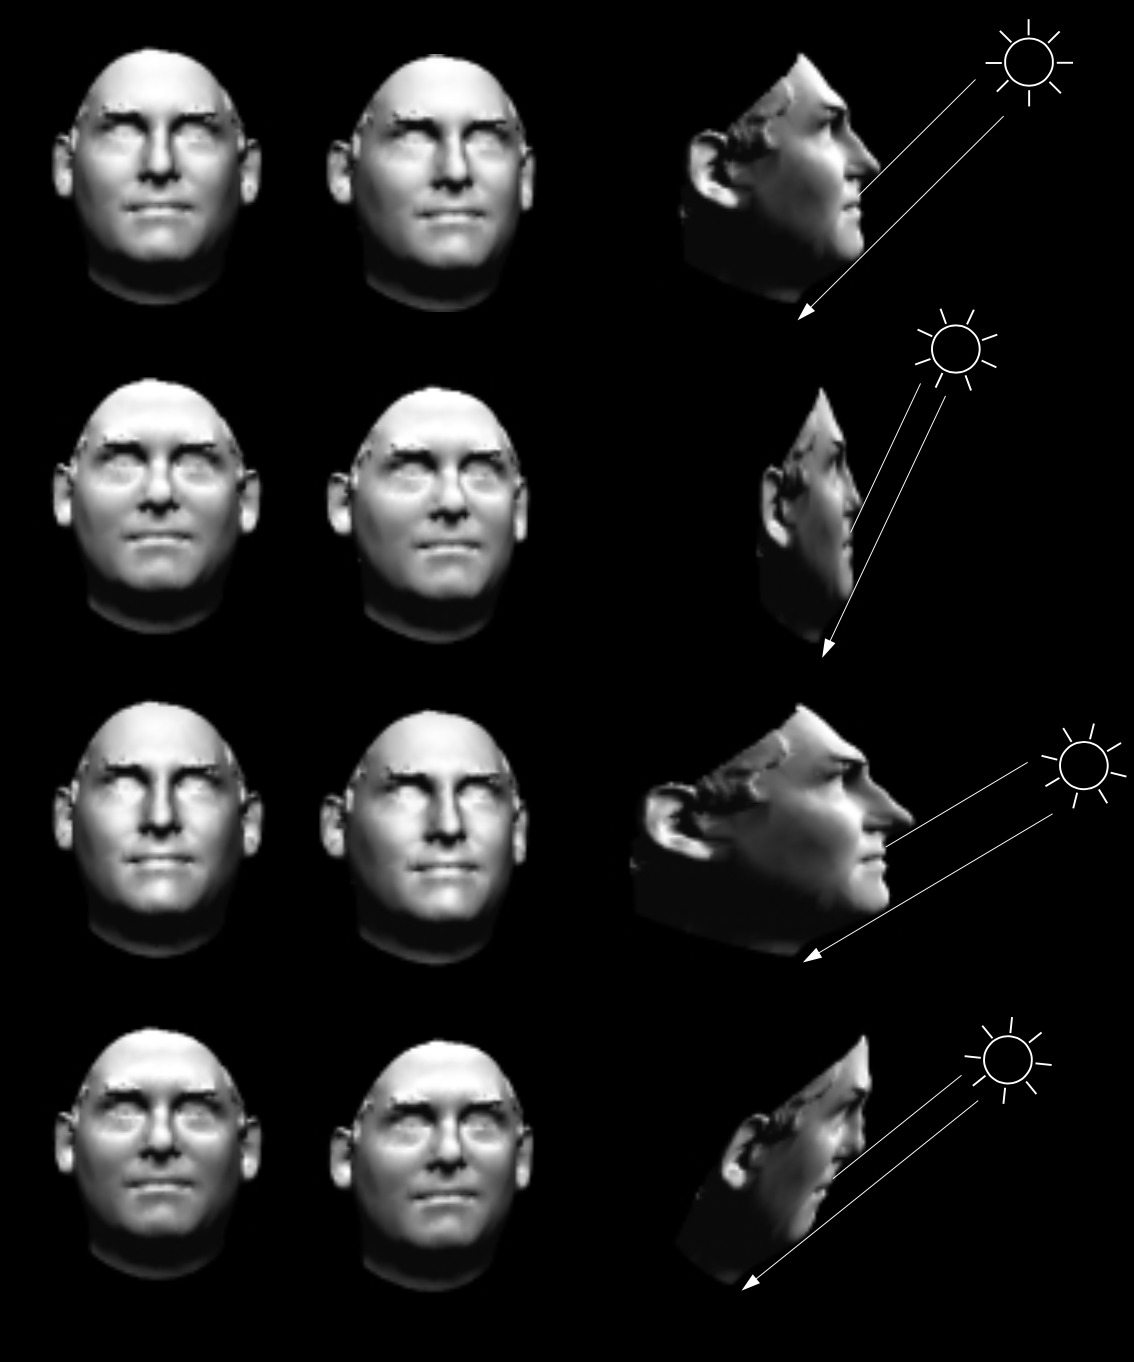
\includegraphics[width=0.6\textwidth]{taxo/gbr.png}
\caption{The effect of GBR ambiguity}
\label{fig:gbr}
\end{figure}

The \textit{reference object} approach, first proposed by~\citeauthor{silver1980determining}, and later revisited by in~\cite{hertzmann2005example}, can be used for surfaces with spatially varying reflectance. The basic assumption is that the BRDF at each point is a linear combination of the ``basis'' BRDFs defined by the set of reference objects.

\section{Class 4}
The dark surface, \ie low reflectance makes any active lighting based technique unsuitable. Thus passive stereo based techniques still work in this case, see Section~\ref{sec:class_3} for details.
\label{sec:class_4}
\begin{table}[h]
  \centering
  \begin{tabular}{l*{3}{c}}
  \hline
  \textbf{Technique} & Textured & Dark & Lambertian\\
  \hline
  SfS & \ding{55} & \ding{55} & \checkmark\\
  MVS & \checkmark & \checkmark & \checkmark\\
  Lamberian PS & \checkmark & \ding{55} & \checkmark\\
  Non Lambertian PS & \checkmark & \ding{55} & \ding{55}\\
  MVPS & \ding{55} & \ding{55} & \checkmark\\
  SL & \ding{55} & \ding{55} & \checkmark\\
  VH & \checkmark & \checkmark & \checkmark\\
  \hline
  \end{tabular}
  \caption{Categories of algorithm that are applicable for object class 4.}
  \label{tab:class_4}
\end{table}

\section{Class 5}
\label{sec:class_5}
\begin{table}[h]
  \centering
  \begin{tabular}{l*{3}{c}}
  \hline
  \textbf{Technique} & Textured & Bright & Non-Lamberian\\
  \hline
  SfS & \ding{55} & \checkmark & \ding{55}\\
  MVS & \checkmark & \checkmark & \ding{55}\\
  Lamberian PS & \checkmark & \checkmark & \ding{55}\\
  Non Lambertian PS & \checkmark & \checkmark & \checkmark\\
  MVPS & \ding{55} & \checkmark & \checkmark\\
  SL & \ding{55} & \checkmark & \ding{55}\\
  VH & \checkmark & \checkmark & \checkmark\\
  \hline
  \end{tabular}
  \caption{Categories of algorithm that are applicable for object class 5.}
  \label{tab:class_5}
\end{table}

\subsection{Non-Lambertian PS: non-uniform reflectance}
One approach exploits the fact that the reflectance of non-Lambertian surfaces can be approximated by \textbf{diffuse component and specular lobe}. \citeauthor{coleman1982obtaining} and \citeauthor{barsky20034} who treat specular pixels as outliers, and \citeauthor{schluns1993photometric}, \citeauthor{sato1994temporal}, and \citeauthor{mallick2005beyond} who assume the color of the specular lobe differs from the color of the diffuse lobe, allowing separation of the specular and diffuse components.

Due to the high complexity of the BRDF, some methods utilize {analytical reflectance models}. \citeauthor{goldman2010shape} uses an isotropic Ward model for each basis BRDF, and the surface orientation and parameters of the reflectance models are estimated iteratively. \citeauthor{alldrin2008photometric} proposed a data-driven approach that got rid of the parametric reflectance model, and employed an novel bi-variate approaximations of isotropic reflectance functions. By combining this approximation with the weighted basis BRDFs, a per-pixel surface normal, global set of non-parametric basis BRDFs, and the corresponding weights are able to be independently estimated. Though the parametric reflectance model can significantly reduce the complexity of BRDFs, they are typically restricted to a limited classes of materials.

Another alternative to using BRDF models is to take advantage of the properties of BRDFs, include energy conservation, non-negativity, Helmholtz reciprocity, or isotropy. Helmholtz stereopsis introduced by~\citeauthor{zickler2002helmholtz} exploits the reciprocity to obtain the surface reconstruction. Isotropy is another physical property which holds for material without ``grain''. \citeauthor{tan2007isotropy} use both symmetry and reciprocity present in isotropic BRDFs to resolve the generalized bas-relief ambiguity. \citeauthor{alldrin2007toward} show that isotropy, with no further assumptions on surface shape or BRDF, can be utilized to recover the surface normal at each surface point up to a plane.
% A four-source photometric stereo technique uses a fourth source of illumination to detecta and remove specular reflections~\cite{coleman1982obtaining}. By adding a fourth image, it's possible to compute four sets of normals, \ie one normal for each permutation of three intensity values. If there is a greater deviation in both magnitude and direction of the normals, a method can now be developed to eliminate specular effects using a thresholding procedure.

\section{Class 6}
\label{sec:class_6}
We discuss textured, mixed diffuse and specular, and bright surface, which is challenging for MVS due to the specular nature, and is difficult for any active techniques since the low amount of reflected light.
\begin{table}[h]
  \centering
  \begin{tabular}{l*{3}{c}}
  \hline
  \textbf{Technique} & Textured & Dark & Non-Lamberian\\
  \hline
  SfS & \ding{55} & \ding{55} & \ding{55}\\
  MVS & \checkmark & \checkmark & \ding{55}\\
  Lamberian PS & \checkmark & \ding{55} & \ding{55}\\
  Non Lambertian PS & \checkmark & \ding{55} & \checkmark\\
  MVPS & \checkmark & \ding{55} & \checkmark\\
  SL & \ding{55} & \ding{55} & \ding{55}\\
  VH & \checkmark & \checkmark & \checkmark\\
  \hline
  \end{tabular}
  \caption{Categories of algorithm that are applicable for object class 6.}
  \label{tab:class_6}
\end{table}

\subsection{VH}
The non-Lambertian property makes any stereo based methods unaviable while the dark surface, or low reflectance makes active lighting methods unsuitable. Thus only visual hull fits in this case, the summary of VH algorithms are listed in Table~\ref{tab:class_6}.
\begin{table}[h]
  \centering
  \begin{tabular}{l*{2}{c}}
  \hline
  \textbf{Technique} & Representation & Algorithm\\
  \hline
  Szeliski~\cite{szeliski1993rapid} & 3D grids & Voxel-based\\
  Tarini~\cite{tarini2002marching} & 3D rays & MI-based\\
  Matusik~\cite{matusik2002efficient} & Polygonal mesh & Exact polyhedral methods\\
  \hline
  \end{tabular}
  \caption{Summary of VH representations and reconstruction approach.}
  \label{tab:summary_class_6}
\end{table}

\section{Summary}
Our taxonomy focuses on the visual cues detected in images, which is utilized by various techniques. Conceptualize these visual cues as dimension of the 3D reconstruction problem, we have an abstraction which allow us to think of algorithms as volumes within a $n-$dimensional problem space. Existing algorithms can be introduced into this framework based on the main visual cue used for reconstruction. Instances where these algorithms have been reported as supporting other forms of variation have been outlined, providing an initial mapping of the space that is summarized below in Table~\ref{tab:algo_taxo}.
\begin{sidewaystable}[h]
  \centering
  \begin{tabular}{l*{6}{c}r}
  \hline
  \textbf{Technique} & Translucency & Texture & Lightness & Reflectance & Roughness & Concavity & \textbf{Class}\\
  Horn~\cite{horn1970shape} & Opaque & Textureless & Bright & Lambertian & N/A & Convex & Class 1\\
  Woodham~\cite{woodham1980photometric} & Opaque & N/A & Bright & Lambertian & N/A & Convex & Class 1, 3\\
  Hayakawa~\cite{hayakawa1994photometric} & Opaque & N/A & Bright & Lambertian & N/A & Convex & Class 1, 3\\
  Belhumeur~\cite{belhumeur1999bas} & Opaque & N/A & Bright & Lambertian & N/A & Convex & Class 1, 3\\
  Coleman~\cite{coleman1982obtaining} & Opaque & N/A & Bright & Non-Lambertian & N/A & Convex & Class 2, 5\\
  Barsky~\cite{barsky20034} & Opaque & N/A & Bright & Non-Lambertian & N/A & Convex & Class 2, 5\\
  Schluns~\cite{schluns1993photometric} & Opaque & N/A & Bright & Non-Lambertian & N/A & Convex & Class 2, 5\\
  Sato~\cite{sato1994temporal} & Opaque & N/A & Bright & Non-Lambertian & N/A & Convex & Class 2, 5\\
  Mallick~\cite{mallick2005beyond} & Opaque & N/A & Bright & Non-Lambertian & N/A & Convex & Class 2, 5\\
  Alldrain~\cite{alldrin2008photometric} & Opaque & N/A & Bright & Non-Lambertian & N/A & Convex & Class 2, 5\\
  Goldman~\cite{goldman2010shape} & Opaque & N/A & Bright & Non-Lambertian & N/A & Convex & Class 2, 5\\
  Silver~\cite{silver1980determining} & Opaque & N/A & Bright & Non-Lambertian & N/A & Convex & Class 1, 2\\
  Hertzmann~\cite{hertzmann2005example} & Opaque & N/A & Bright & Non-Lambertian & N/A & Convex & Class 1, 2, 3, 5\\
  Zickler~\cite{zickler2002helmholtz} & Opaque & N/A & Bright & Non-Lambertian & N/A & Convex & Class 3, 5\\
  Furukawa~\cite{furukawa2010accurate} & Opaque & Textured & N/A & Lambertian & N/A & Convex & Class 3, 4\\
  Goesele~\cite{goesele2006multi} & Opaque & Textured & N/A & Lambertian & N/A & Convex & Class 3, 4\\
  Vogiatzis~\cite{vogiatzis2007multiview} & Opaque & Textured & N/A & Lambertian & N/A & Convex & Class 3, 4\\
  Szeliski~\cite{szeliski1993rapid} & Opaque & N/A & N/A & N/A & N/A & Convex & Class 1-6\\
  Tarini~\cite{tarini2002marching} & Opaque & N/A & N/A & N/A & N/A & Convex & Class 1-6\\
  Matusik~\cite{matusik2002efficient} & Opaque & N/A & N/A & N/A & N/A & Convex & Class 1-6\\
  \hline
  \end{tabular}
  \caption{Algorithm classification based on the new taxonomy}
  \label{tab:algo_taxo}
\end{sidewaystable}